\begin{frame}
  \frametitle{Canonical discriminant HE plots}

	\begin{itemize}
		\item As with biplot, we can visualize MLM hypothesis variation for
		\emph{all} responses by projecting \H and \E into low-rank space.
		\item \alert{Canonical projection}:
		$ \mat{Y}_{n \times p}  \implies
		  \mat{Z}_{n \times s} = \mat{Y} \mat{E}^{-1/2} \mat{V}
		$, where $\mat{V}$ = eigenvectors of $\H \inv{E}$.
		\item This is the view that maximally discriminates among groups, ie max. \H wrt \E!

	\end{itemize}
  \begin{center}	
  \includegraphics<1>[width=.85\textwidth,clip]{fig/gcaniris}
  \end{center}	

\end{frame}

\begin{frame}
  \frametitle{Canonical discriminant HE plots}

	\begin{itemize}
		\item Canonical HE plot is just the HE plot of canonical scores,
		$(\vec{z}_1, \vec{z}_2)$ in 2D,
		\item or, $\vec{z}_1, \vec{z}_2, \vec{z}_3,$ in 3D.
		\item As in biplot, we add vectors to show relations of the
		$\vec{y}_i$ response variables to the canonical variates.
		\item variable vectors here are \alert{structure coefficients} = 
		correlations of variables with canonical scores.
	\end{itemize}
	
  \begin{center}	
  \includegraphics<1>[width=.85\textwidth,clip]{fig/hecaniris}
  \end{center}	
\end{frame}

\begin{frame}
  \frametitle{Canonical discriminant HE plots: Properties}

	\begin{itemize}
	  \item Canonical variates are uncorrelated: \E ellipse is spherical
	  \item $\implies$ axes must be equated to preserve geometry
%	  \item Circles of radius \(\sqrt { \chi_2^2 ( 1 -\alpha  ) /  n_i }\) give confidence regions for group means.
	  \item Variable vectors show how variables discriminate among groups
	  \item Lengths of variable vectors $\sim$ contribution to discrimination
	\end{itemize}
	
  \begin{center}	
  \includegraphics<1>[width=.85\textwidth,clip]{fig/hecaniris}
  \end{center}	
\end{frame}

\begin{frame}<\inlong>
  \frametitle{Canonical discriminant HE plots}
	\begin{itemize}
		\item Can also visualize canonical dimensions in variable space
	\end{itemize}
    \begin{center}
  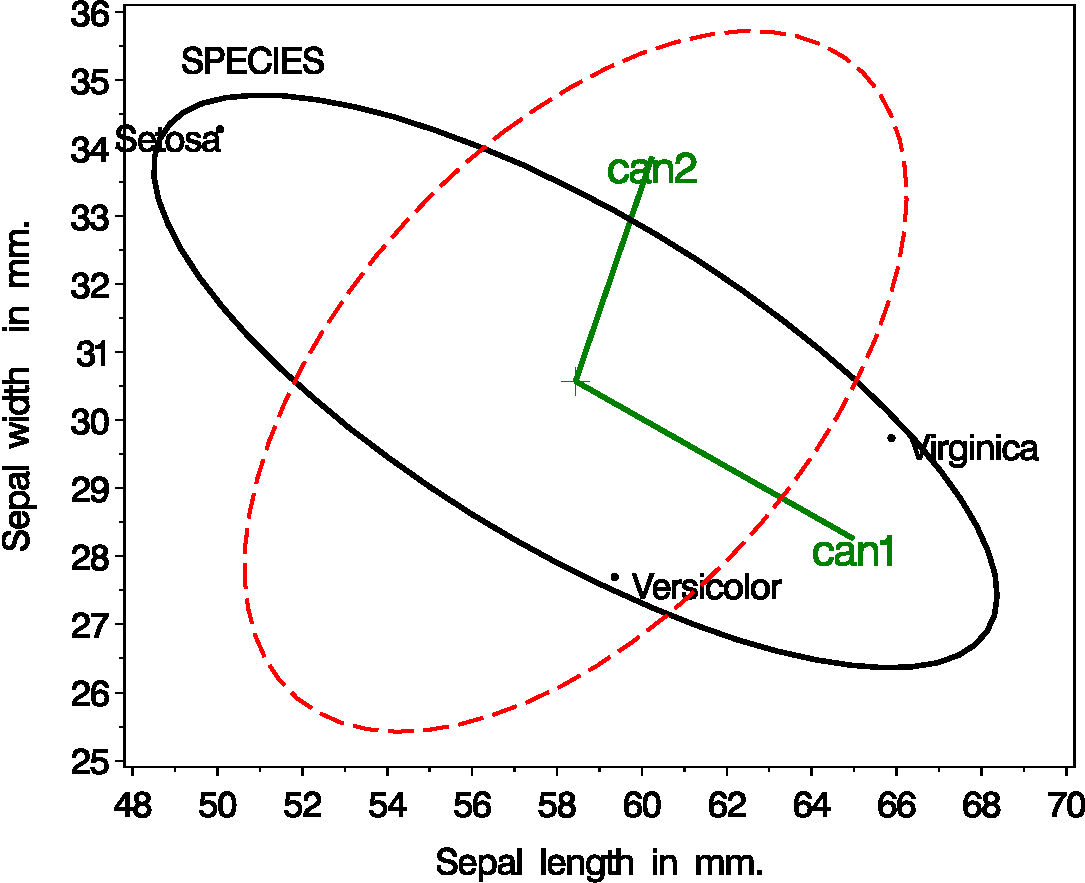
\includegraphics[width=.7\textwidth,clip]{fig/hematiris-can2}
    \end{center}
\end{frame}
\begin{frame}<\inlong>
  \frametitle{Canonical discriminant HE plots}
	\begin{itemize}
		\item $\dots$ and for all response varaiables
	\end{itemize}
    \begin{center}
  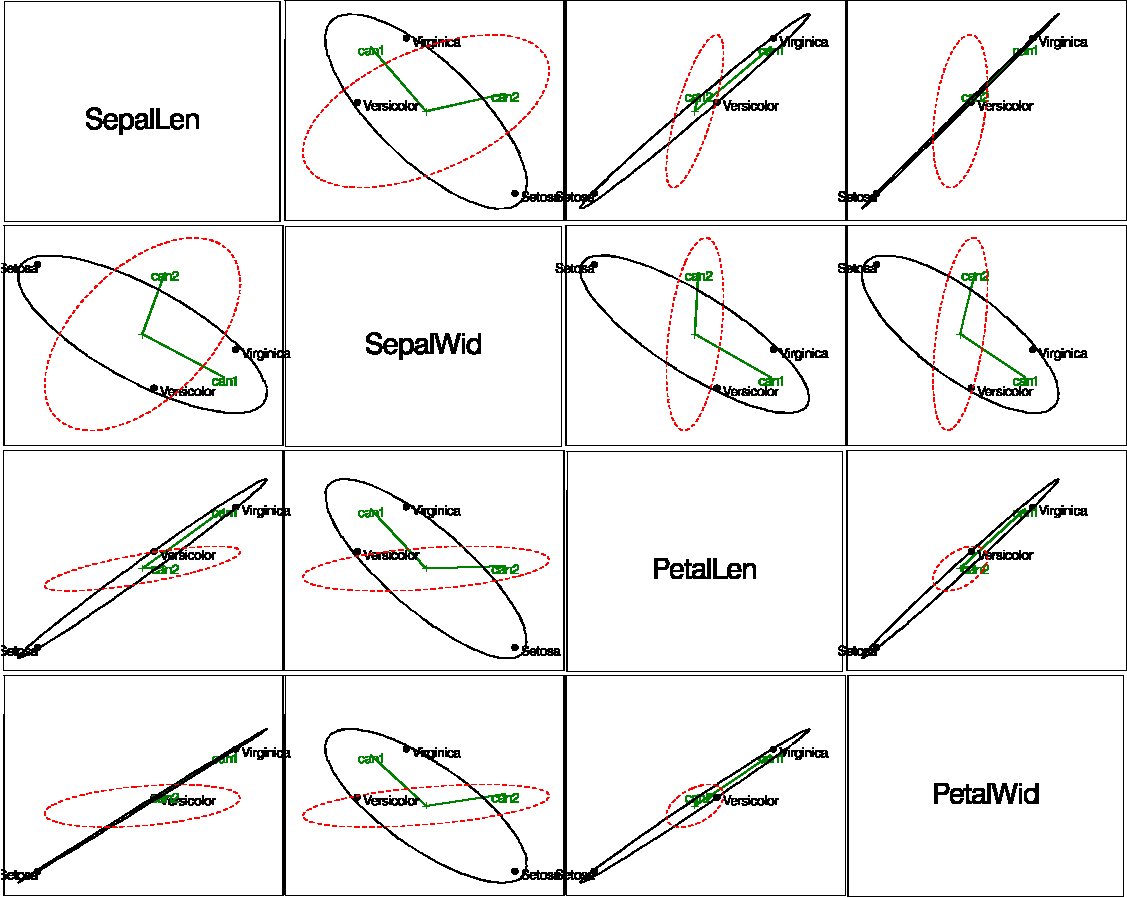
\includegraphics[width=.7\textwidth,clip]{fig/hematiris-can1}
    \end{center}
\end{frame}

\begin{frame}
  \frametitle{Canonical discriminant HE plots: Pottery data}

	\begin{itemize}
	  \item Canonical HE plots provide 2D (3D) visual summary of \H vs. \E variation
	  \item Pottery data: $p=5$ variables, 4 groups \implies $df_H=3$
	  \item Variable vectors: Fe, Mg  and Al contribute to distingiushing (Caldicot,
	  Llandryn) from (Isle Thorns, Ashley Rails): 96.4\% of mean variation
	  \item Na and Ca contribute an additional 3.5\%.  \alert{End of story!}
	\end{itemize}
	
  \begin{center}	
  \includegraphics<1>[width=.85\textwidth,clip]{fig/pottery-can1}
  \end{center}	
  \href{run:powerpoint.bat}{\beamerbutton{Run heplot-movie.ppt}}
\end{frame}

